As an extra phase to the project and as a beginning of the future work for this project, we've tried to improve the performance of the Translation Cache implementation.

The Dynamic Binary Translator is a complex system and the performance of the system depends critically on how the translation process is done. 
When a new Basic Block (BB) translation is initiated, the \textbf{DBTEngine checks} if the BB is already translated. The TCache will answer NULL if it's not translated or will answer with the address of the translated code if it's translated. 

In the Implementation Phase we show two different ways of implementing th TCache:
\begin{itemize}
	\item Single Translation - This method reduces the overhead but forces the DBT to translate every time that the actual BB is not the last translated BB because this method only saves the last translation;
	\item Multiple Translation - This implementation allows the DBT to store multiple translations, producing more overhead but in compensation it's more efficient because the DBT needs to translate the code less times in comparison with the Single Translation method. The additional overhead of this method is caused by the recursive algorithm of searching in the Hash Table.
\end{itemize}

Since the Hash Table is most efficient software, we've tried to add an extra objective to this project: recurring to the Hardware Offloading, implement the TCache component in hardware.

For this implementation, there are five main phases:
\begin{enumerate}
	\item Choose the FPGA and get used to the specific protocol of communication between hardware peripherals.
	\item Decide the implementation of the TCache. As aforementioned in the design phase, this implementation has 2 alternatives:
	\begin{itemize}
		\item TCache (Content Addressable Memory module and Random Access Memory module);
		\item Only Content Addressable Memory module.
	\end{itemize}
	\item Decide if the hardware module should have an LITE or FULL interface;
	\item Run the Dynamic Binary Translator in the selected FPGA;
	\item Integrate the implemented module with the DBT software in the selected FPGA.
\end{enumerate}

As mentioned in the design phase, the chosen development board is the Zynq - 7000 Development Board from Digilent because it contains the processor ARM Cortex-A9 that is compatible with the Thumb2 which is the architecture of ours supervisor board. Besides that, the zynq board is integrated in the board catalog of Vivado Design Suite from Xilinx. Vivado allows the user to create IP modules and connect them using the AXI protocol.

Since the board and the communication protocol is already defined, the next step is to define how the TCache will be implemented. Using the Vivado Design Suite, we develop the TCache fully in hardware, as illustrated in figure \ref{fig:HwError1}. 

\begin{figure} [h!]
	\centering
	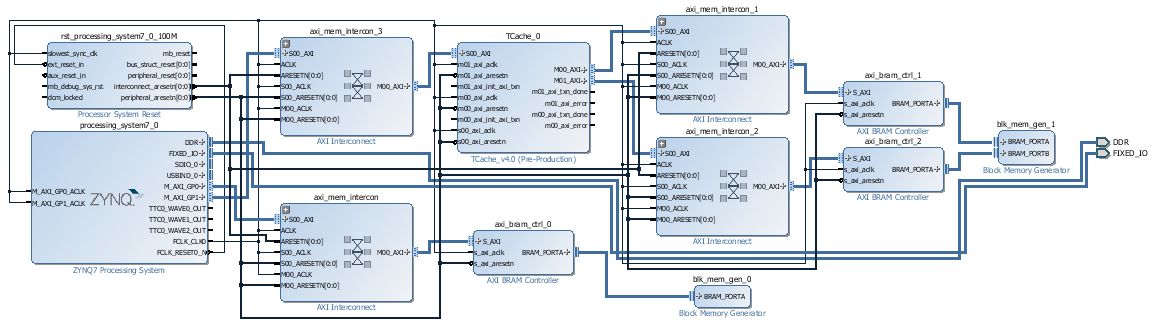
\includegraphics[scale = 0.45]{Images/HwError1.png}
	\caption{Translation Cache hardware implementation}
	\label{fig:HwError1}
\end{figure}

In parallel with this implementation we've developed a CAM in hardware, illustrated in the figure \ref{fig:CAM_Hw}.

\begin{figure} [H]
	\centering
	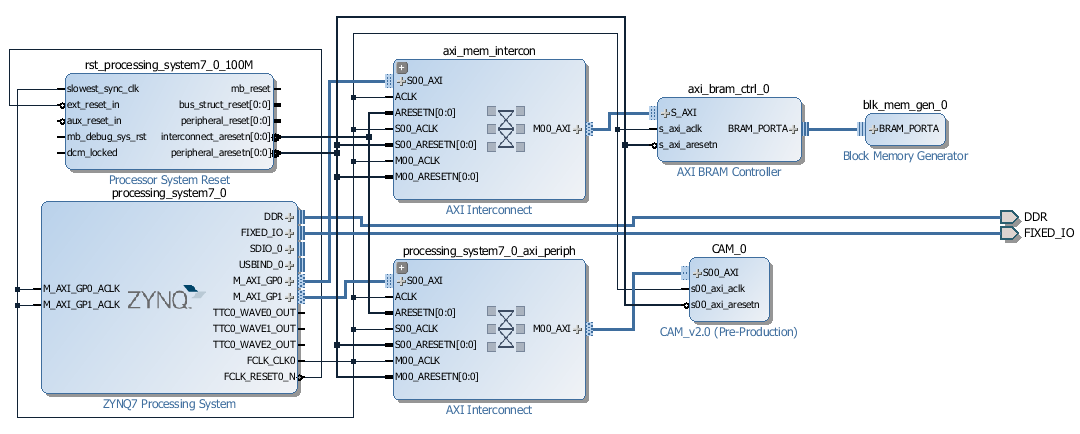
\includegraphics[scale = 0.45]{Images/CAM_Hw.png}
	\caption{CAM hardware implementation}
	\label{fig:CAM_HwImp}
\end{figure}

The main difference between them is that the TCache includes a CAM and a RAM, and the second implementation is only a CAM, as aforementioned in the design phase.
In the first implementation the translated code is stored by the TCache in the RAM. In the second implementation, the translated code is store by the ZYNQ in the DDR3 memory using a DDR3 DMA controller.

When using the AXI, the fully implementation of the TCache in hardware will introduce to much overhead because for each instruction translated, the ZYNQ would have to initiate a AXI LITE connection and send the translated instruction to the TCache and the TCache would have to do the same with the BRAM controller.

The solution is to reduce this overhead is to implement only the CAM in hardware and store the translated code in the DDR3 Memory through the DDR3 DMA controller. The flow of DBTEngine will be like the flow in the figure \ref{fig:flow}. 

After deciding the implementation of the TCache, it's now necessary to decide if the implemented module will have AXI FULL or LITE interface. They are quite similar but the AXI FULL contains more signals in order to allow bursts of data. A burst is a set of N data transfers (beats) where each beat can be a number of M bytes. Both N and M variables are defined every time the connection is opened. 

Since the DBT only translates and stores one instruction at a time, the AXI FULL is not ideal for this module. The AXI LITE has less overhead and it is ideal for this application because with the LITE the module can only exchange 1 word at a time. The size of the word is configured every time a connection is opened. The disadvantaged of this interface is that every time the DBT translates something, it will have to initiate the connection, introducing overhead. However, this is the suitable option for this implementation.

\begin{figure} [H]
	\centering
	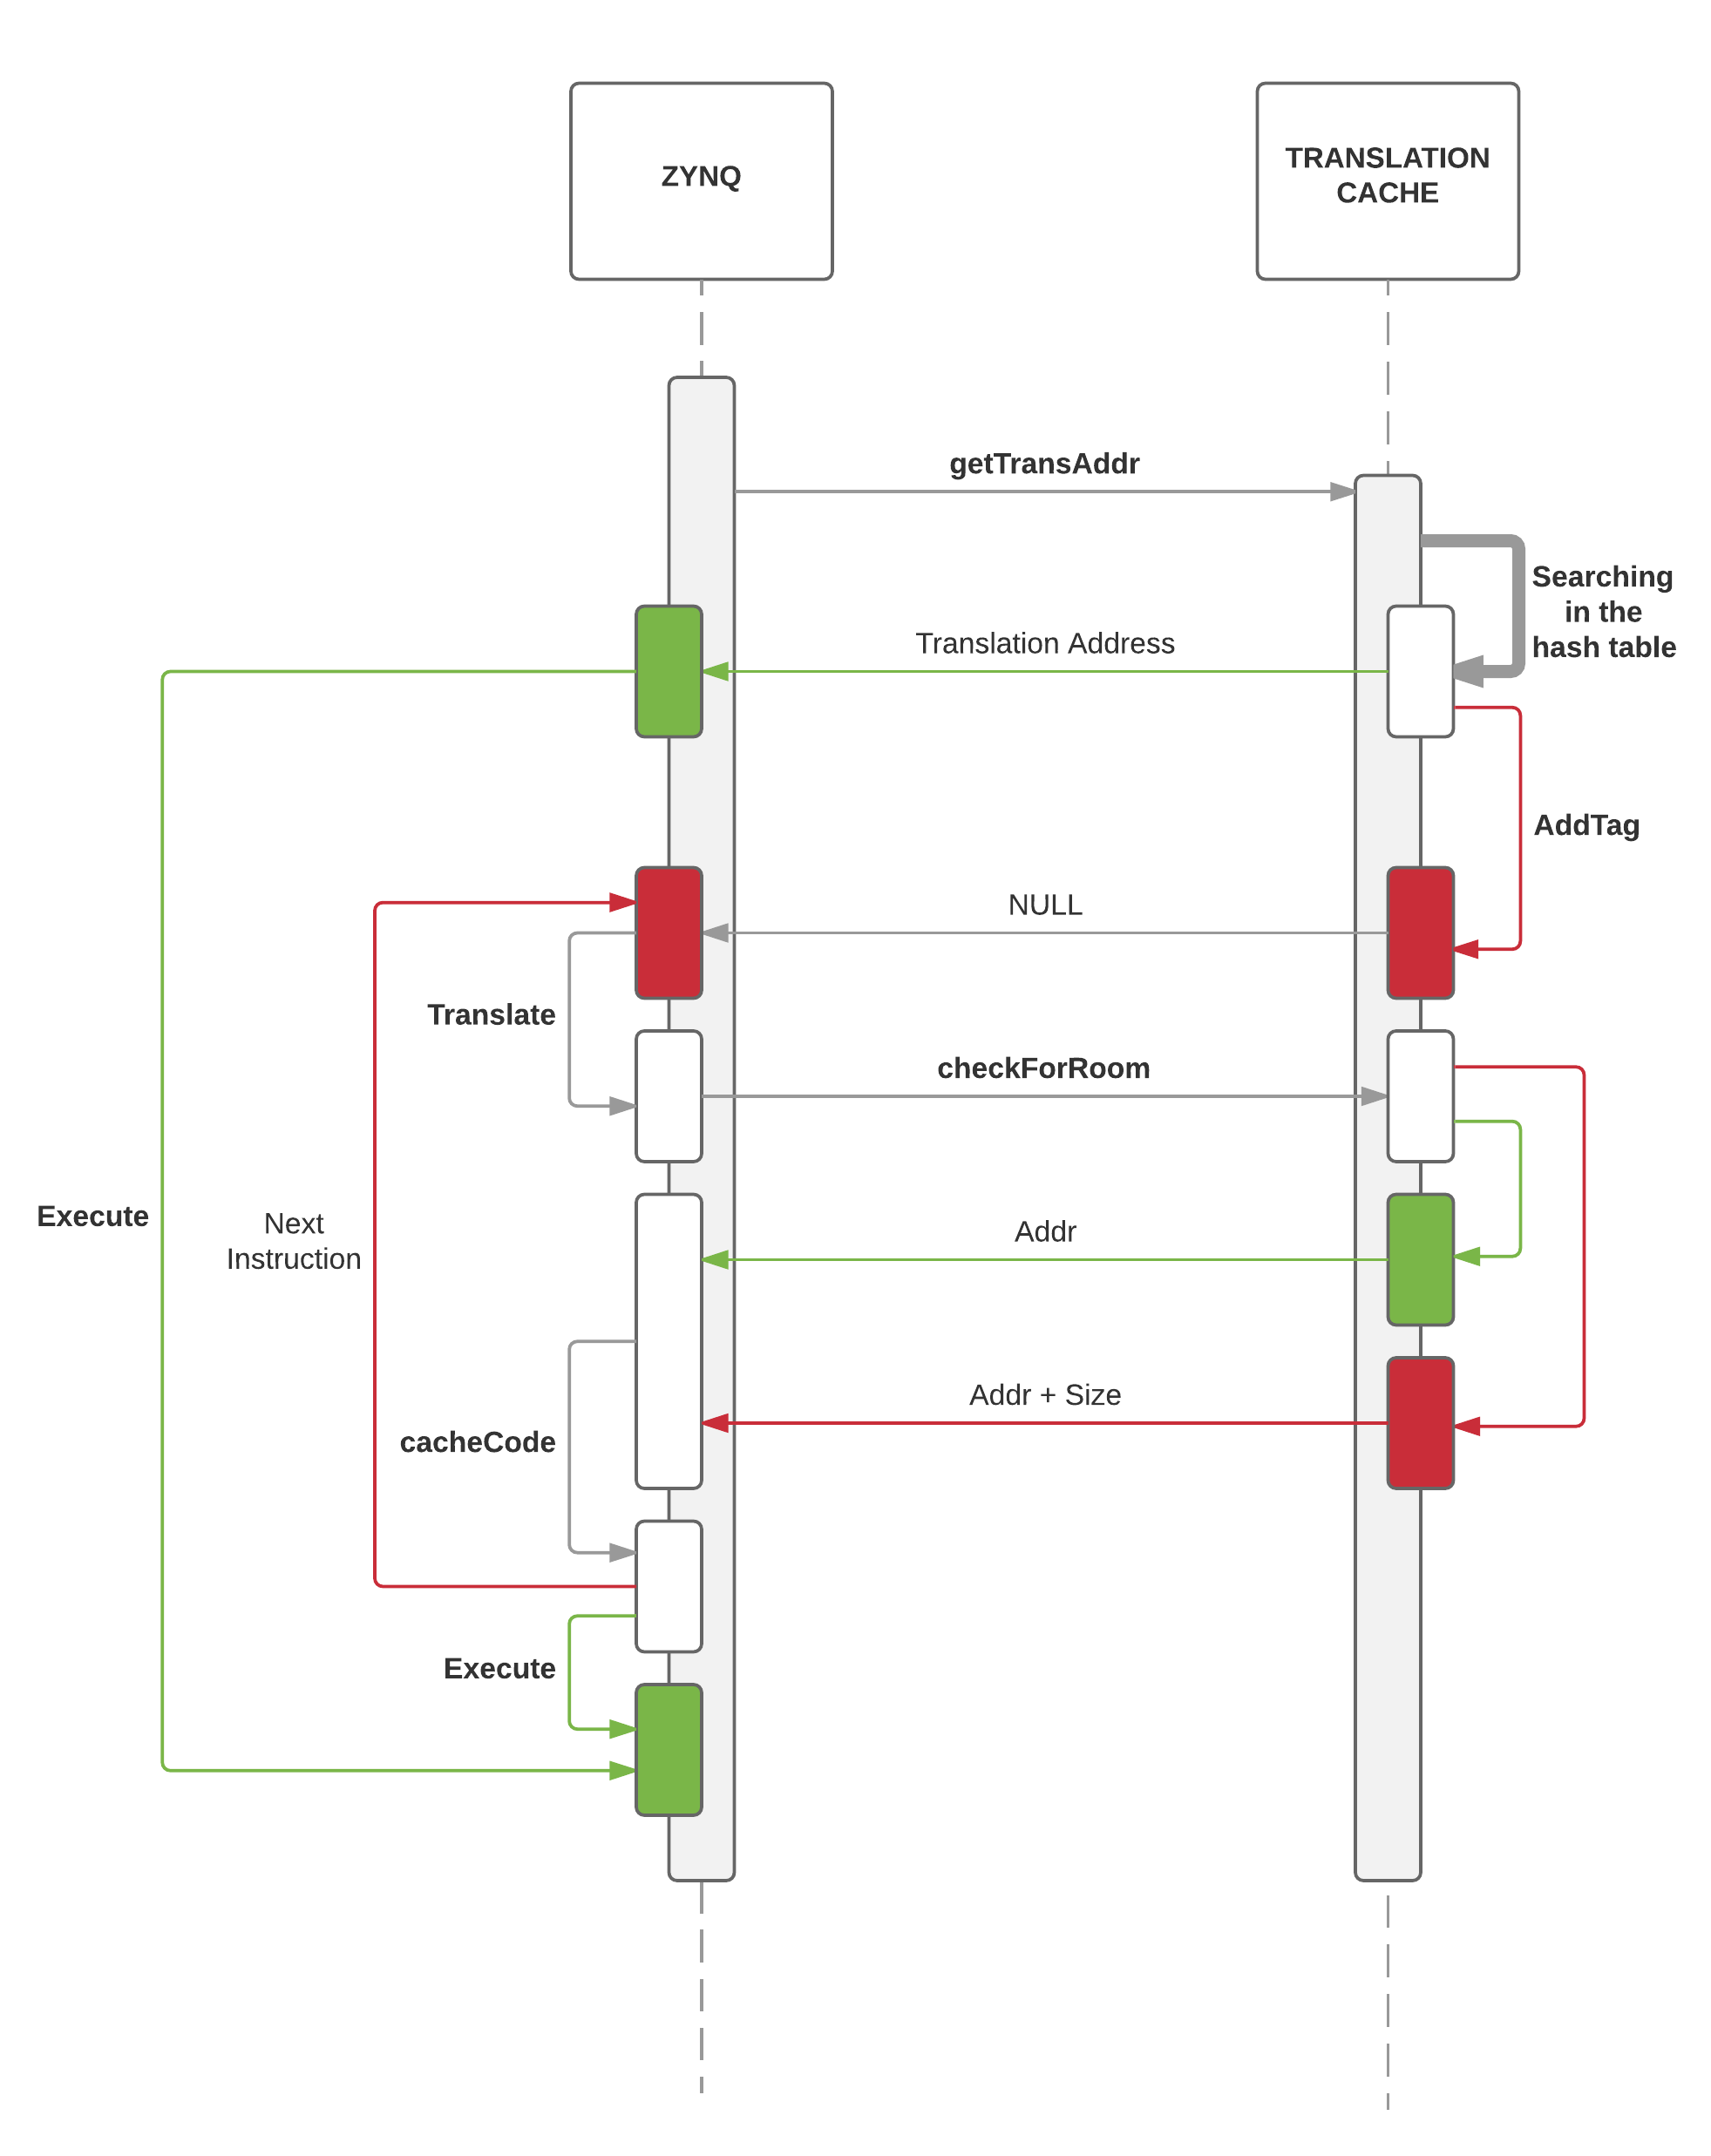
\includegraphics[scale = 0.12]{Images/flow.png}
	\caption{Flow of execution in the DBTEngine}
	\label{fig:flow}
\end{figure}
